As we have seen in chapter~\ref{chap:benchmark_results}, evaluation of Learning-to-Rank methods is spread out over the several benchmark datasets. However, as the evaluated Learning-to-Rank methods differ from benchmark to benchmark, no single benchmark comparison can be regarded as a conclusive argument on which Learning-to-Rank method is most accurate.\\

Several studies make a small start in considering Learning-to-Rank method performance over multiple benchmark datasets. Gomes et al. \cite{Gomes2013} analysed ranking accuracy of a set of models over both LETOR 3.0 and LETOR 4.0. Busa-Fekete et al. \cite{Busa-Fekete2013} compared the accuracy of a small set of models over the LETOR 4.0 datasets, both MSLR datasets, both Yahoo! Learning to Rank Challenge datasets and the OHSUMED dataset from LETOR 3.0. To my knowledge, no large-scale accuracy meta-analysis has been conducted where published evaluation results on several benchmark datasets are taken into account. With a meta-analysis I will compare the performance of Learning-to-Rank methods across the Learning-to-Rank benchmark datasets described in foregoing sections.

\section{Collecting Evaluation Results}
With a literature review I will collect evaluation results on the datasets/collections. The following list presents an overview of the benchmark collections taken into account in the meta-analysis:
\begin{itemize}
\item LETOR 2.0
\item LETOR 3.0
\item LETOR 4.0
\item Yahoo! Learning to Rank Challenge
\item Yandex Internet Mathematics Competition 2009
\item MSLR-web10/30k
\item WCL2R
\item AOL
\end{itemize}

For the LETOR collections, the evaluation results of the baseline models will be used from LETOR 2.0\footnote{http://research.microsoft.com/en-us/um/beijing/projects/letor/letor2.0/baseline.aspx}, LETOR 3.0\footnote{http://research.microsoft.com/en-us/um/beijing/projects/letor/letor3baseline.aspx} and LETOR 4.0\footnote{http://research.microsoft.com/en-us/um/beijing/projects/letor/letor4baseline.aspx} as listed on the LETOR website.\\

LETOR 1.0, LETOR 3.0, Yahoo! Learning to Rank Challenge, WCL2R and AOL have an accompanying paper that was published together with the benchmark collection. Users of those benchmark collections are encouraged to cite these papers. A forward literature search on these studies is performed to collect studies that present measurements of evaluations of Learning-to-Rank methods on these benchmark collections. Table~\ref{tbl:ltr_benchmark_forref} presents an overview of the results of this forward literature search.

\begin{table}[!h]
\begin{tabular}{l|l|l}
Benchmark & Paper & \# of forward references \\
\hline
LETOR 1.0 \& 2.0 & Liu et al. \cite{Liu2007b} & 307\\
LETOR 3.0 & Qin et al. \cite{Qin2010} & 105\\
Yahoo! Learning to Rank Challenge & Chapelle et al. \cite{Chapelle2011a} & 102\\
AOL dataset & Pass et al. \cite{Pass2006} & 339\\
WCL2R & Alc{\^a}ntara et al. \cite{Alcantara2010} & 2\\
\end{tabular}
\caption{Forward references of Learning-to-Rank benchmark papers}
\label{tbl:ltr_benchmark_forref}
\end{table}

The LETOR 4.0, MSLR-web10/30k and Yandex Internet Mathematics Competition 2009 benchmark collections were not accompanied with a describing study. To collect measurements of Learning-to-Rank methods evaluated on these benchmarks, a Google Scholar search is performed on the name of the benchmark. Table~\ref{chap:benchmark_results} shows the results of this literature search.

\begin{table}[!h]
\begin{tabular}{l|l}
Benchmark & Google scholar search results \\
\hline
LETOR 4.0 & 75 results \\
MSLR-web10k & 16 results \\
MSLR-web30k & 15 results \\
Yandex Internet Mathematics Competition & 1 result \\ 
\end{tabular}
\caption{Google scholar search results for Learning-to-Rank benchmarks}
\label{tbl:ltr_benchmark_searchres}
\end{table}

\section{Comparison Methodology}
The LETOR 3.0 paper \cite{Qin2010} states that it may differ between datasets what the most accurate ranking methods are. To evaluate the overall performance of Learning-to-Rank methods over the multiple datasets in the LETOR 3.0 collections, Qin et al. \cite{Qin2010} proposed a measure called \emph{winning number} as the number of other algorithms that an algorithm can beat over the set of datasets. Formally the winning number measure is defined as\\

$\text{Winning Number}_i(M) = \sum\nolimits_{j=1}^n \sum\nolimits_{k=1}^m I_{\{M_i(j)>M_k(j)\}}$\\

where $j$ is the index of a dataset, $n$ the number of datasets in the comparison, $i$ and $k$ are indices of an algorithm, $M_i(j)$ is the performance of the $i$-th algorithm on the $j$-th dataset, $M$ is a ranking measure (such as \ac{nDCG} or \ac{MAP}), and $I_{\{M_i(j)>M_k(j)\}}$ is an indicator function such that\\

$I_{\{M_i(j)>M_k(j)\}} = \begin{cases}
1 & \text{if } M_i(j) > M_k(j), \\
0 & \text{otherwise}
\end{cases}$\\

In contrast to the winning number comparison on LETOR 3.0, there will not be accuracy measurements for each algorithm on each dataset in our meta-analysis. To compare algorithms based on a sparse set of evaluation measurements, a normalised version of the winning number metric will be used which we calculate by only taking those datasets into account that an algorithm is evaluated on and then dividing this by the ideal winning number that an algorithm could have had if it would have been the best algorithm on all datasets on which it has been evaluated. I will redefine the indicator function $I$ in order to only take into account those datasets that an algorithm is evaluated on, as \\

$I_{\{M_i(j)>M_k(j)\}} = \begin{cases}
1 & \text{if } M_i(j) \text{ and } M_k(j) \text{ are both defined and } M_i(j) > M_k(j), \\
0 & \text{otherwise}
\end{cases}$\\

From now on this adjusted version of winning number will be references to as \emph{normalised winning number}. The mathematical definition of normalised winning number is\\

$\text{Normalised Winning Number}_i(M) = \frac{\text{Winning Number}_i(M)}{\text{Ideal Winning Number}_i(M)}$\\

\noindent
where ideal winning number is defined as\\

$\text{Ideal Winning Number}_i(M) = \sum\nolimits_{j=1}^n \sum\nolimits_{k=1}^m D_{\{M_i(j),M_k(j)\}}$\\

where $j$ is the index of a dataset, $n$ the number of datasets in the comparison, $i$ and $k$ are indices of an algorithm, $M_i(j)$ is the performance of the $i$-th algorithm on the $j$-th dataset, $M$ is a ranking measure (such as \ac{nDCG} or \ac{MAP}), and $D_{\{M_i(j),M_k(j)\}}$ is an evaluation definition function such that\\

$D_{\{M_i(j),M_k(j)\}} = \begin{cases}
1 & \text{if } M_i(j) \text{ and } M_k(j) \text{ are both defined}, \\
0 & \text{otherwise}
\end{cases}$\\

\section{Evaluation Results Found in Literature}
\begin{table}[!h]
\scalebox{0.85}{
\begin{tabular}{|l|l|l||l|l|l|}
Method & Described & Evaluated & Method & Described & Evaluated \\
\hline 
AdaRank-\acs{MAP} & \cite{Xu2007} &  & Linear Regression &  & \cite{Wang2012, Volkovs2011} \\ 
AdaRank-\acs{nDCG} & \cite{Xu2007} & \cite{Busa-Fekete2013,Tan2013} & List\acs{MLE} &  & \cite{Lin2010, Lin2011, Gao2014} \\ 
ADMM & \cite{Duh2011} & \cite{Duh2011} & ListNet &  &  \\ 
Approx\acs{AP} & \cite{Qin2010b} & \cite{Qin2010b} & ListReg & \cite{Wu2011} & \cite{Wu2011} \\ 
Approx\acs{nDCG} & \cite{Qin2010b} & \cite{Qin2010b} & LRUF & \cite{Torkestani2012b} & \cite{Torkestani2012b} \\ 
BagBoo & \cite{Pavlov2010} & \cite{Ganjisaffar2011c} & MCP & \cite{Laporte2013} & \cite{Laporte2013} \\ 
Best Single Feature &  & \cite{Gomes2013} & MHR &  &  \\ 
BL-MART & \cite{Ganjisaffar2011c} & \cite{Ganjisaffar2011c} & MultiStageBoost & \cite{Kao2013} & \cite{Kao2013} \\ 
BoltzRank-Single & \cite{Volkovs2009} & \cite{Volkovs2009} & NewLoss & \cite{Peng2010} & \cite{Peng2010} \\ 
BoltzRank-Pair & \cite{Volkovs2009} & \cite{Volkovs2009, Ganjisaffar2011c} & OWPC & \cite{Usunier2009} & \cite{Usunier2009} \\ 
BT & \cite{Zhou2008} & \cite{Zhou2008} & PERF-\acs{MAP} &  & \cite{Torkestani2012b} \\ 
C-\acs{CRF} & \cite{Qin2008b} & \cite{Qin2008b} & PermuRank & \cite{Xu2008} & \cite{Xu2008} \\ 
CA & \cite{Metzler2007} & \cite{Busa-Fekete2013,Tan2013} & Q.D.\acs{KNN} &  & \cite{Wang2013} \\ 
CCRank & \cite{Wang2011c} & \cite{Wang2011c} & RandomForest &  & \cite{Gomes2013} \\ 
CoList & \cite{Gao2014} & \cite{Gao2014} & Rank-PMBGP & \cite{Sato2013} & \cite{Sato2013} \\ 
Consistent-RankCosine &  & \cite{Tan2013} & RankAgg\acs{nDCG} & \cite{Wang2013} & \cite{Wang2013} \\ 
DCMP & \cite{Renjifo2012}  & \cite{Renjifo2012}  & RankBoost &  & \cite{Busa-Fekete2013} \\ 
DirectRank & \cite{Tan2013} & \cite{Tan2013} & RankCSA & \cite{He2010} & \cite{He2010} \\ 
Energy\acs{nDCG} & \cite{Freno2011} & \cite{Freno2011} & RankDE &  & \cite{Sato2013} \\ 
FBPCRank & \cite{Lai2011} & \cite{Lai2011} & RankELM (pairwise) & \cite{Zong2013} & \cite{Zong2013} \\ 
FenchelRank & \cite{Lai2013} & \cite{Lai2013, Lai2013b, Laporte2013} & RankELM (pointwise) & \cite{Zong2013} & \cite{Zong2013} \\ 
FocusedBoost & \cite{Niu2012} & \cite{Niu2012} & RankMGP & \cite{Lin2012} & \cite{Lin2012} \\ 
FocusedNet & \cite{Niu2012} & \cite{Niu2012} & RankNet &  & \cite{Busa-Fekete2013, Papini2012, Niu2012} \\ 
Focused\acs{SVM} & \cite{Niu2012} & \cite{Niu2012} & Rank\acs{RLS} &  &  \\ 
FP-Rank & \cite{Song2013} & \cite{Song2013} & Rank\acs{SVM} &  & \cite{Busa-Fekete2013, Freno2011, He2010} \\ 
FRank &  & \cite{Wang2012} & Rank\acs{SVM}-Primal &  & \cite{Lai2011} \\ 
FSMRank & \cite{Lai2013c} & \cite{Lai2013c,Laporte2013} & Rank\acs{SVM}-Struct &  &  \\
FSM$^{\acs{SVM}}$ & & \cite{Lai2013c} & RCP & \cite{Elsas2008} & \cite{Elsas2008} \\ 
GAS-E &  & \cite{Lai2013c} & RE-QR & \cite{Veloso2010} & \cite{Veloso2010} \\ 
\acs{GP}Rank & \cite{Silva2009} & \cite{Torkestani2012} & REG-SHF-SDCG & \cite{Wu2009} & \cite{Wu2009} \\ 
GRank\acs{RLS} & \cite{Pahikkala2010} & \cite{Pahikkala2010} & Ridge Regression &  &  \\ 
Group\acs{CE} & \cite{Lin2011} & \cite{Lin2011} & RSRank &  & \cite{Lai2013} \\ 
Group\acs{MLE} & \cite{Lin2010} & \cite{Lin2011} & SmoothGrad &  & \cite{Tan2013} \\ 
IntervalRank & \cite{Moon2010} & \cite{Moon2010, Freno2011} & SmoothRank & \cite{Chapelle2010} & \cite{Chapelle2010} \\ 
\acs{IP}Rank & \cite{Wang2009b} & \cite{Wang2009b, Torkestani2012} & SoftRank &  & \cite{Qin2010b} \\ 
KeepRank & \cite{Chen2009} & \cite{Chen2009} & SortNet & \cite{Rigutini2008} & \cite{Rigutini2008,Freno2011} \\ 
Kernel-\acs{PCA} RankBoost & \cite{Duh2008} & \cite{Duh2008, Sato2013} & SparseRank & \cite{Lai2013b} & \cite{Lai2013b} \\ 
KL-\acs{CRF} & \cite{Volkovs2011} & \cite{Volkovs2011} & \acs{SVD}-RankBoost & \cite{Lin2009} & \cite{Lin2009} \\ 
LAC-MR-OR & \cite{Veloso2008} & \cite{Veloso2008} & \acs{SVM}$^{\acs{MAP}}$ &  & \cite{Wang2012, Xu2008, Niu2012} \\ 
LambdaMART & \cite{Burges2010} & \cite{Asadi2013a, Ganjisaffar2011c} & SwarmRank &  & \cite{Sato2013} \\ 
LambdaNeuralRank & \cite{Papini2012} & \cite{Papini2012} & TGRank &  & \cite{Lai2013} \\ 
LambdaRank &  &  & TM & \cite{Zhou2008} & \cite{Zhou2008, Papini2012, Tan2013} \\ 
LARF & \cite{Torkestani2012} & \cite{Torkestani2012} & VFLR & \cite{Cai2012} & \cite{Cai2012} \\ 
\end{tabular}}
\caption{Learning-to-Rank algorithms with measurements on benchmark datasets}
\label{ltr_methods_used}
\end{table}

\section{Results \& Discussion}
\subsection{MAP}

\subsection{NDCG@3}

\subsection{NDCG@5}

\subsection{NDCG@10}

\subsection{All metrics}
\begin{figure}[!h]
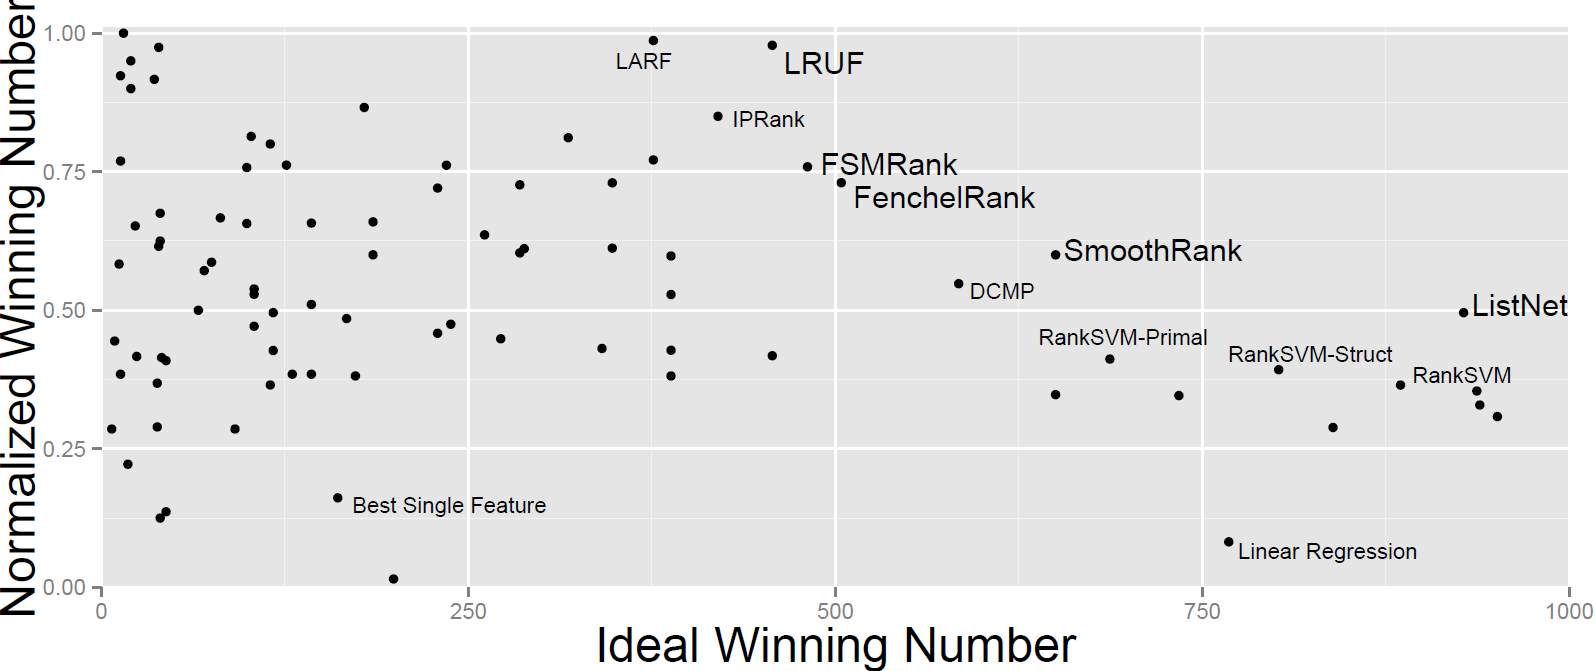
\includegraphics[scale=0.40]{gfx/combined_normalized_winnum}
\caption{Cross-benchmark comparison of Learning-to-Rank methods}
\label{fig:normalised_winning_number_all}
\end{figure}
%TODO: waarom ndcg@3,5,10 en MAP?
%TODO: limitations van deze vergelijkingsmethodologie

\section{Limitations}